\documentclass[9pt,xcolor=dvipsnames]{beamer}
\usetheme{Warsaw}
\usepackage[utf8]{inputenc}
\usepackage[english]{babel}
\usepackage[T1]{fontenc}
\usepackage{amsmath}
\usepackage{amsfonts}
\usepackage{amssymb}
\usepackage{graphicx}

\definecolor{Vert}{RGB}{116,185,44}
\definecolor{Bleu}{RGB}{31,29,108}


\setbeamercolor{frametitle}{bg=Vert}
\setbeamercolor{framenumber}{bg=Bleu,fg=white}
\setbeamerfont{page number in head/foot}{size=\large}
\setbeamercolor{structure}{fg=Vert!90!black}

\setbeamertemplate{footline} {
  \leavevmode%
  \hbox{%
  \begin{beamercolorbox}[wd=.4\paperwidth,ht=2.25ex,dp=1ex,center]{author in head/foot}%
    \usebeamerfont{author in head/foot}\insertshortauthor
  \end{beamercolorbox}%
  \begin{beamercolorbox}[wd=.5\paperwidth,ht=2.25ex,dp=1ex,center]{title in head/foot}%
    \usebeamerfont{title in head/foot}\insertshorttitle\hspace*{3em}
  \end{beamercolorbox}}%
  \begin{beamercolorbox}[wd=.1\paperwidth,ht=2.25ex,dp=1ex,center]{framenumber}
     \usebeamerfont{framenumber}\insertframenumber{} / \inserttotalframenumber\hspace*{1ex}
  \end{beamercolorbox}%
  \vskip0pt%
}

\pgfdeclareimage[height=0.6cm]{logo}{../img/paquito.png}
\logo{\pgfuseimage{logo}}

\author{Paquiteam}
\title{Détail des cas d'utilisation}
\subtitle{Paquito, easy packaging}


\date{26 janvier 2016} 

\begin{document}

\begin{frame}
\titlepage
\end{frame}

\section*{La Paquiteam}
\begin{frame}{La Paquiteam}
	\begin{center}
		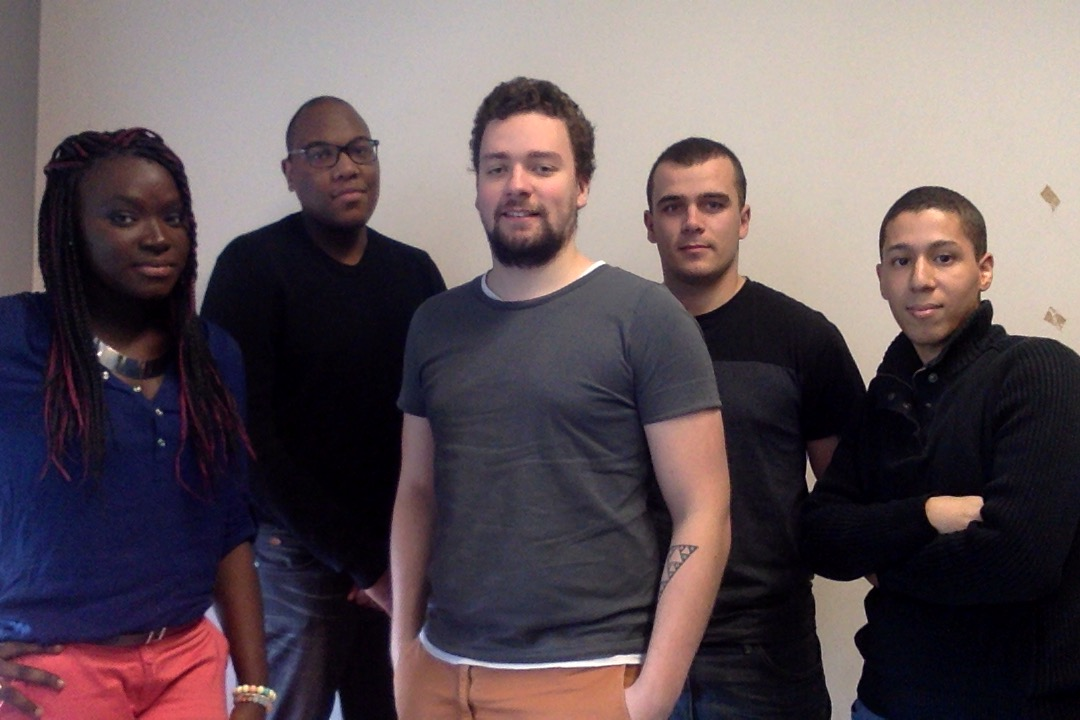
\includegraphics[scale=0.26]{../img/paquiteam.jpg}
	\end{center}
\end{frame}


\begin{frame}
\tableofcontents
\end{frame}

\newcommand\largeur{0.15}

\section{Cas d'utilisation}
\subsection{Diagramme des cas d'utilisation}
\begin{frame}{Diagramme des cas d'utilisation}
  \begin{center}	
    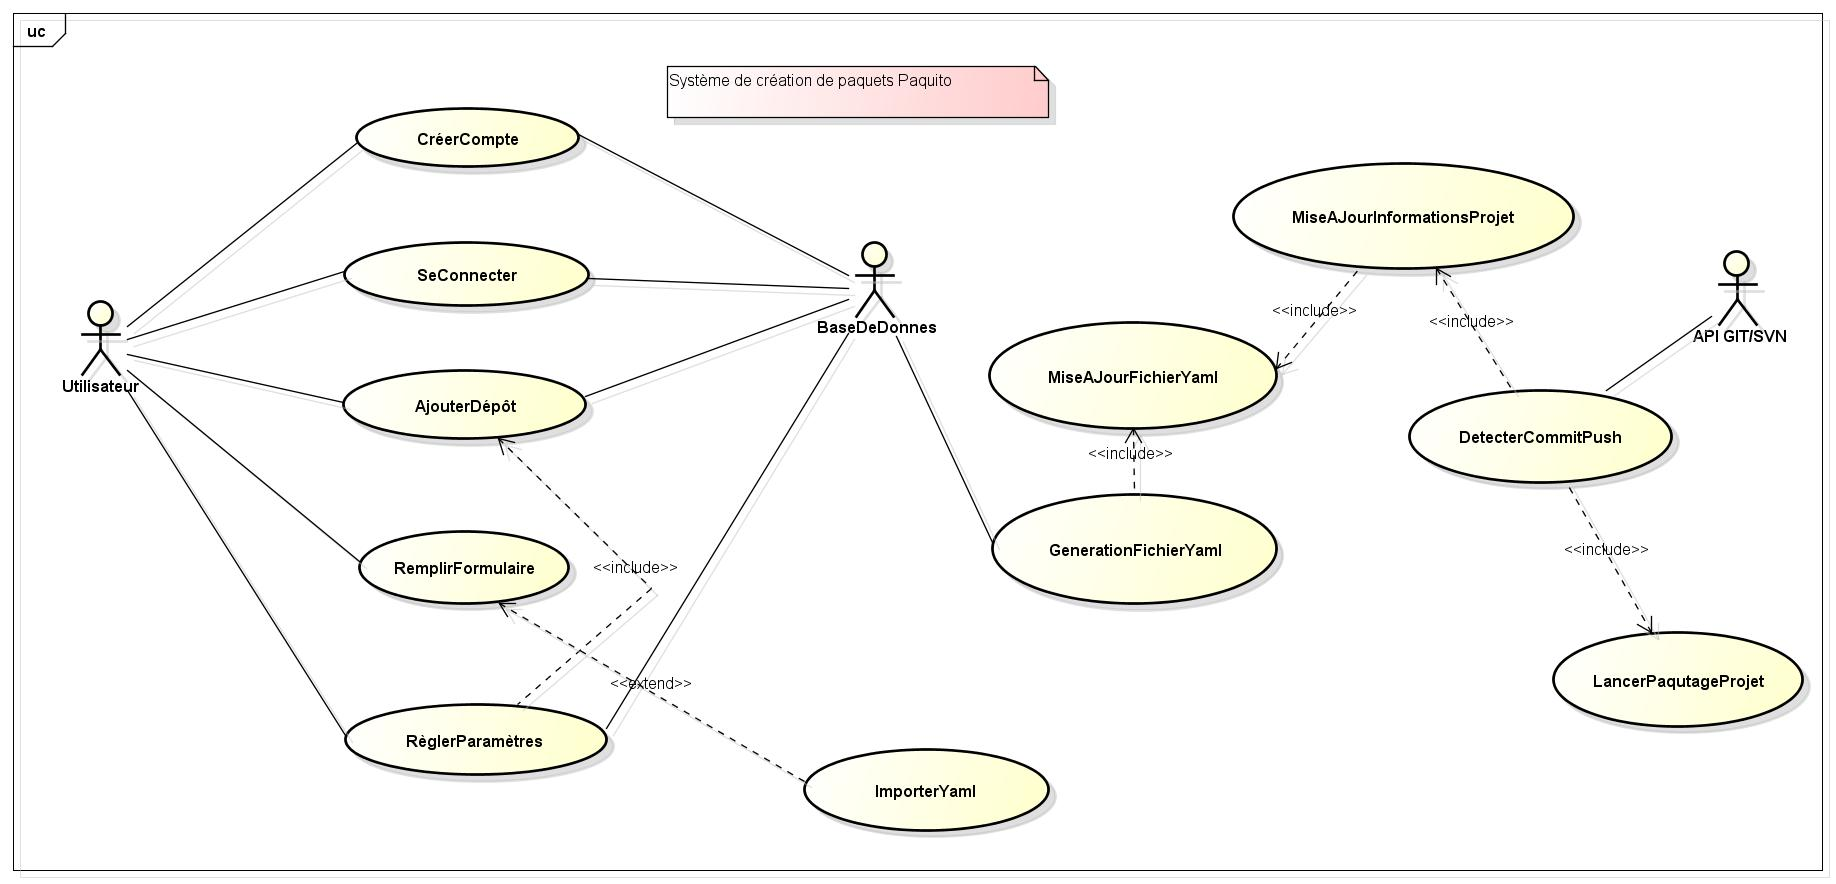
\includegraphics[scale=0.15]{../img/Diagram1.jpg}
  \end{center}
\end{frame}

\subsection{Détail des cas d'utilisation}
\begin{frame}{Créer un compte}
  \begin{minipage}{0.40\textwidth}
    \begin{flushleft}
      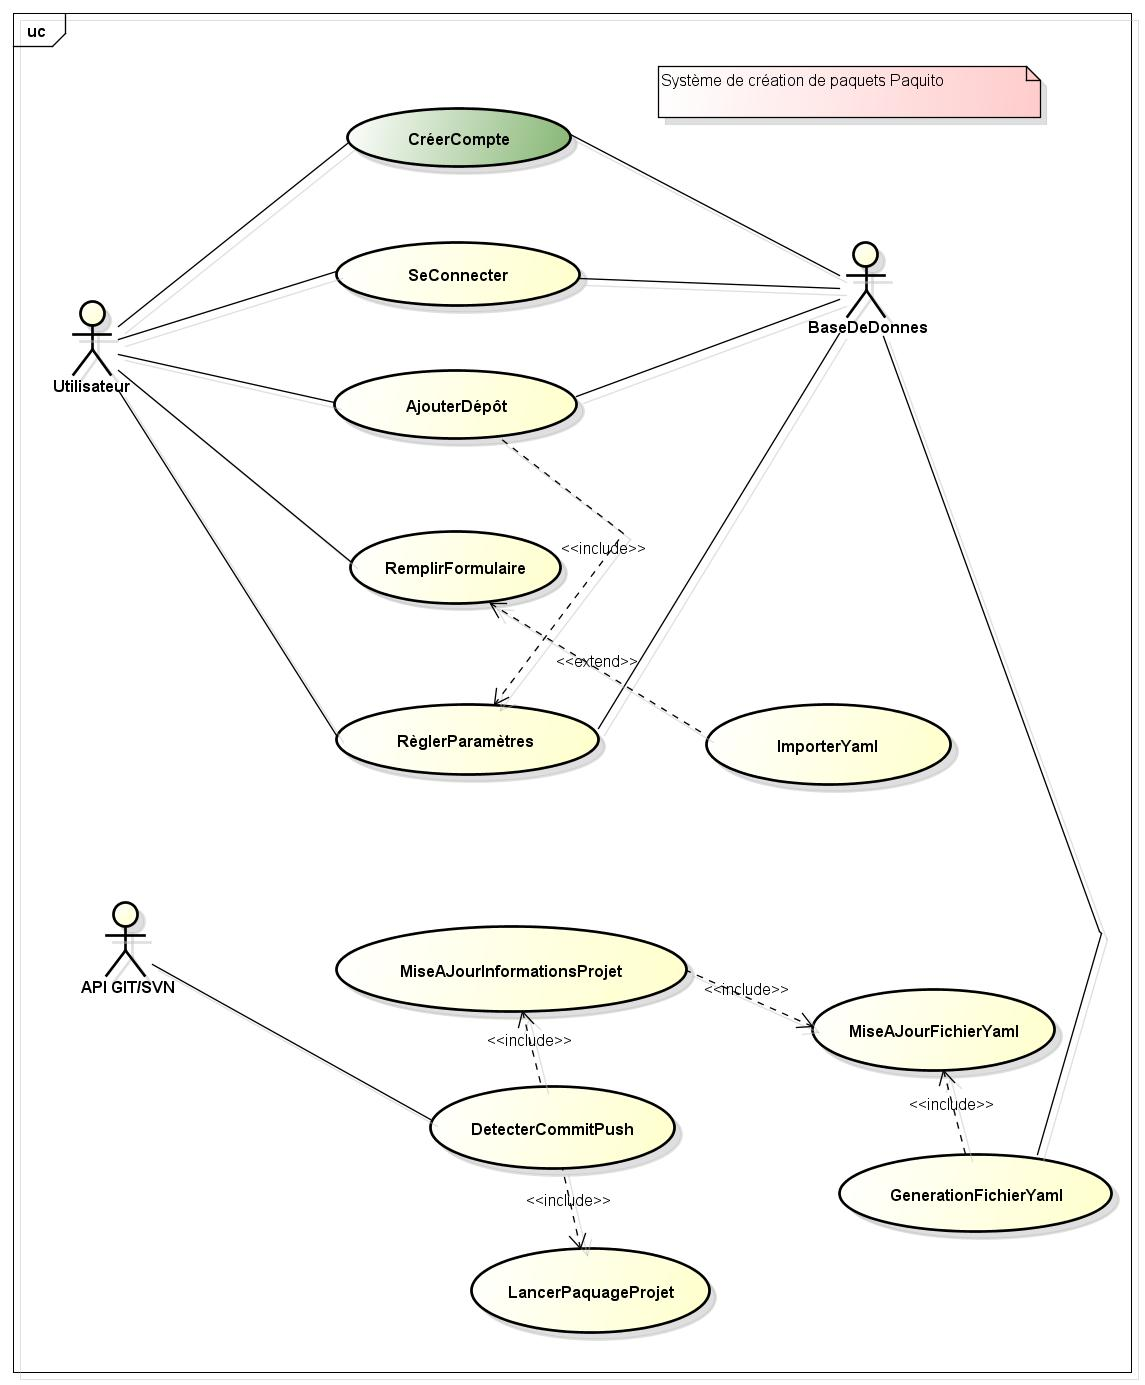
\includegraphics[scale=\largeur]{../img/Diagram_creerCompte.jpg}
    \end{flushleft}
  \end{minipage}
  \hfill
  \begin{minipage}{0.5\textwidth}
    \begin{flushright}
      \begin{itemize} 
      \item \textbf{Identification} 
        \begin{itemize} 
        \item[] Niveau de l'action : Sous-fonction 
        %\item[] But : L'utilisateur (le développeur) crée un compte pour utiliser le service Web 
        \item[] Acteur : Utilisateur 
        \end{itemize} 
      \item \textbf{Scénario principal} 
        \begin{enumerate} 
        \item L'utilisateur renseigne ses coordonnées 
        \item Le site web accepte l'inscription 
        \end{enumerate}
      \end{itemize}
    \end{flushright}
  \end{minipage}
\end{frame}

\begin{frame}{Se connecter}
  \begin{minipage}{0.40\textwidth}
    \begin{flushleft}
      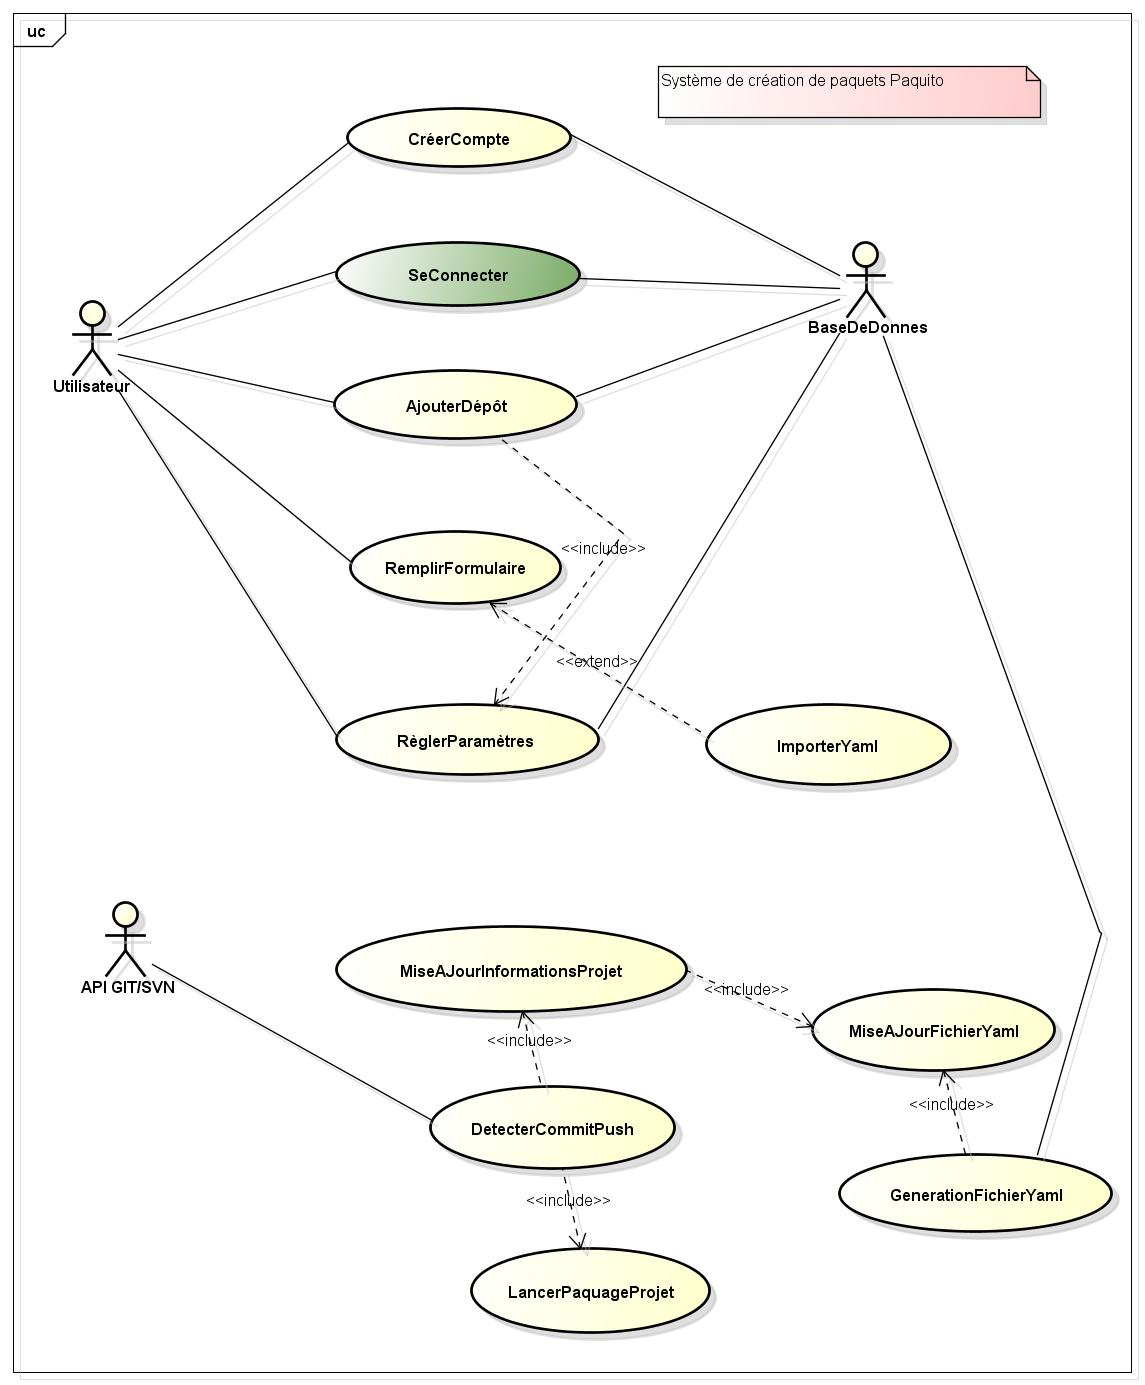
\includegraphics[scale=\largeur]{../img/Diagram_seConnecter.jpg}
    \end{flushleft}
  \end{minipage}
  \hfill
  \begin{minipage}{0.5\textwidth}
    \begin{flushright}
      \begin{itemize} 
      \item \textbf{Identification} 
        \begin{itemize} 
        \item[] Niveau de l'action : Sous-fonction 
        %\item[] But : L'utilisateur (le développeur) se connecte pour utiliser le service Web
        \item[] Acteur : Utilisateur 
        \end{itemize} 
      \item \textbf{Scénario principal} 
        \begin{enumerate} 
        \item L'utilisateur entre son login et son mot de passe 
        \item Le site web accepte l'inscription 
        \end{enumerate} 
      \item \textbf{Echec} 
        \begin{enumerate} 
        \item L'utilisateur n'est pas inscrit 
        \item Le site web notifie l'erreur et propose à l'utilisateur de s'inscrire 
        \item L'utilisateur est inscrit mais n'a pas renseigné le bon mot de passe 
        \item Le site web notifie l'erreur et propose à l'utilisateur de recommencer 
        \end{enumerate} 
      \end{itemize}
    \end{flushright}
  \end{minipage}
\end{frame}

\begin{frame}{Ajouter un dépôt}
  \begin{minipage}{0.40\textwidth}
    \begin{flushleft}
      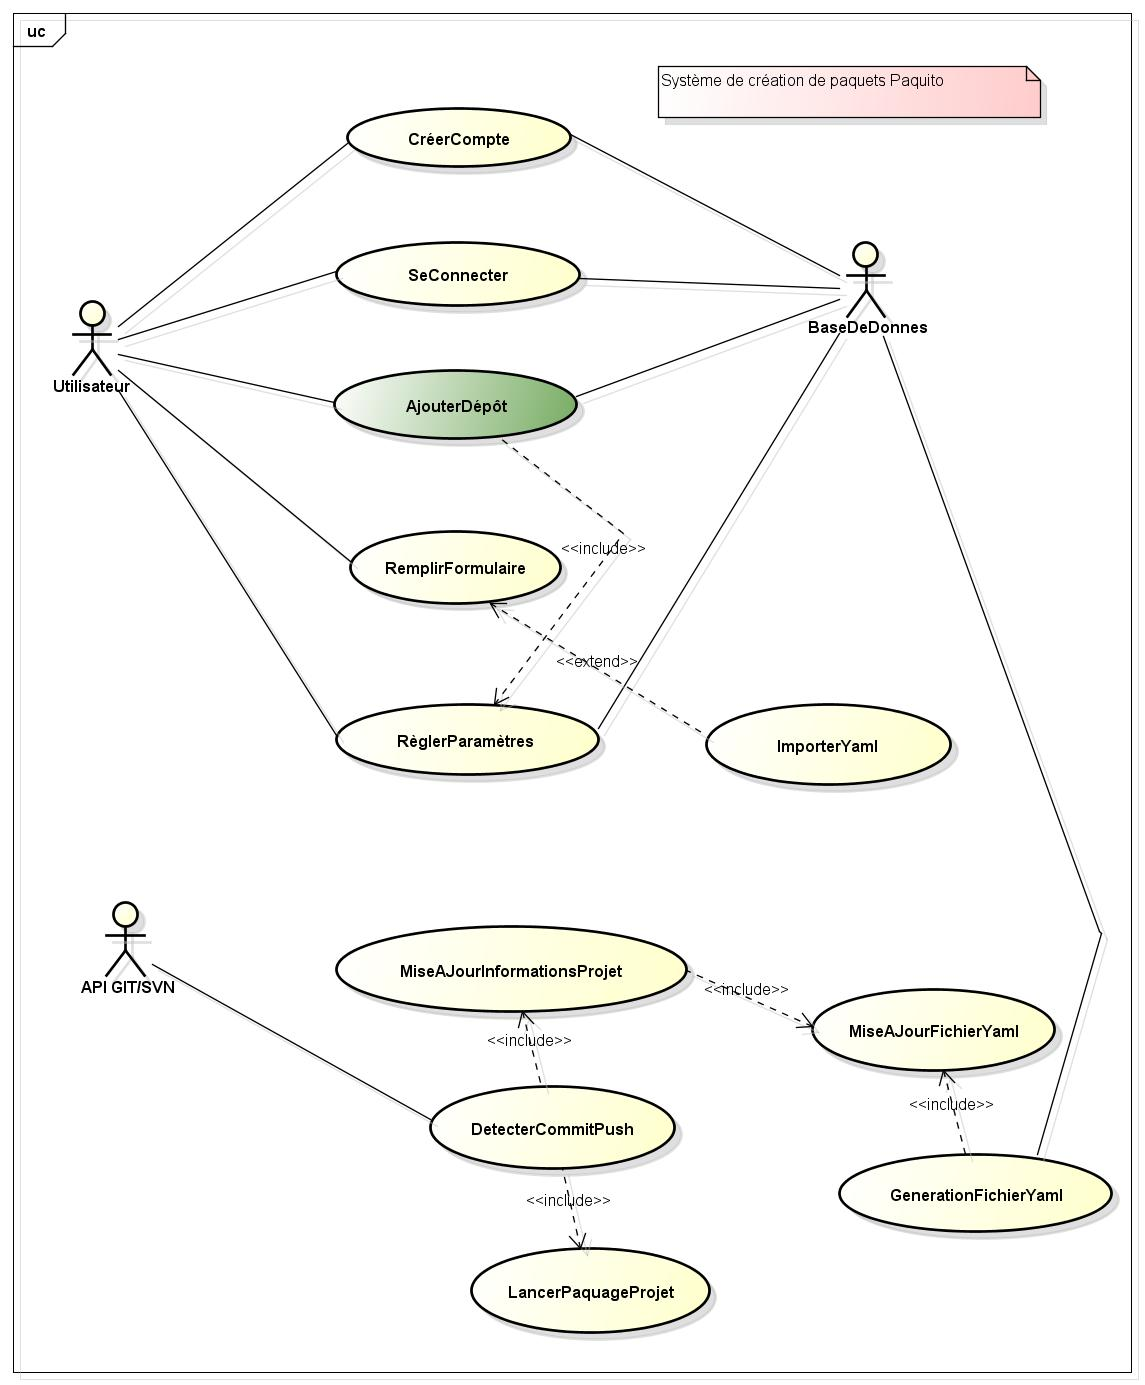
\includegraphics[scale=\largeur]{../img/Diagram_ajouterDepot.jpg}
    \end{flushleft}
  \end{minipage}
  \hfill
  \begin{minipage}{0.5\textwidth}
    \begin{flushright}
      \begin{itemize} 
      \item \textbf{Identification} 
        \begin{itemize} 
        \item[] Niveau de l'action : But utilisateur 
        %\item[] But : Le développeur ajoute un dépôt sur le service Web pour un projet.
        \item[] Acteur : Utilisateur 
        \end{itemize} 
      \item \textbf{Scénario principal} 
        \begin{enumerate} 
        \item L'utilisateur indique le nom et l'URL du dépôt. 
        \item Le serveur est contacté et lance la commande d'ajout de dépôt. 
        \end{enumerate} 
      \end{itemize}
    \end{flushright}
  \end{minipage}
\end{frame}

\begin{frame}{Mise à jour des informations du projet}
  \begin{minipage}{0.40\textwidth}
    \begin{flushleft}
      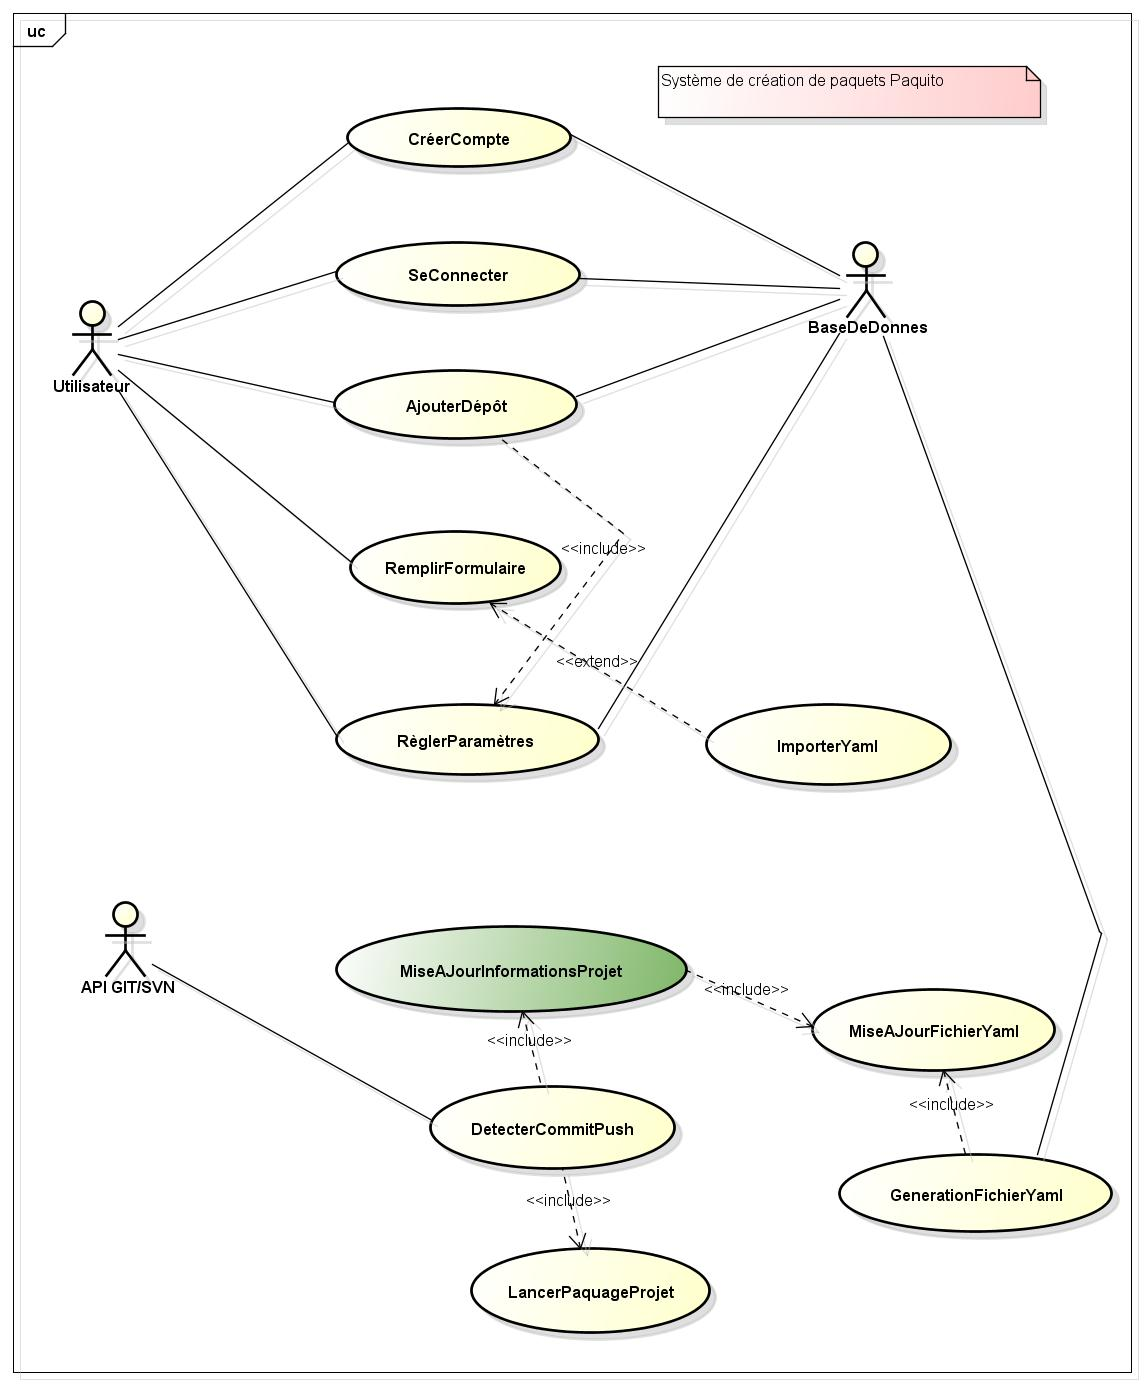
\includegraphics[scale=\largeur]{../img/Diagram_miseAJourInformationsProjet.jpg}
    \end{flushleft}
  \end{minipage}
  \hfill
  \begin{minipage}{0.5\textwidth}
    \begin{flushright}
      \begin{itemize}
      \item \textbf{Identification}
        \begin{itemize}
        \item[] Niveau de l'action : Sous fonction
        %\item[] But : Mettre à jour les informations du projet
        \item[] Acteur : Utilisateur
        \end{itemize}
      \item \textbf{Scénario principal}
        \begin{enumerate}
        \item Le développeur change les informations via l'application web
        \item Les informations sont changées suite à un commit ou un push
        \item Changement des informations dans la Base de Donnée
        \item Génération du nouveau fichier YAML
        \end{enumerate}
      \end{itemize}
    \end{flushright}
  \end{minipage}
\end{frame}

\begin{frame}{Régler paramètres de création de paquets}
  \begin{minipage}{0.40\textwidth}
    \begin{flushleft}
      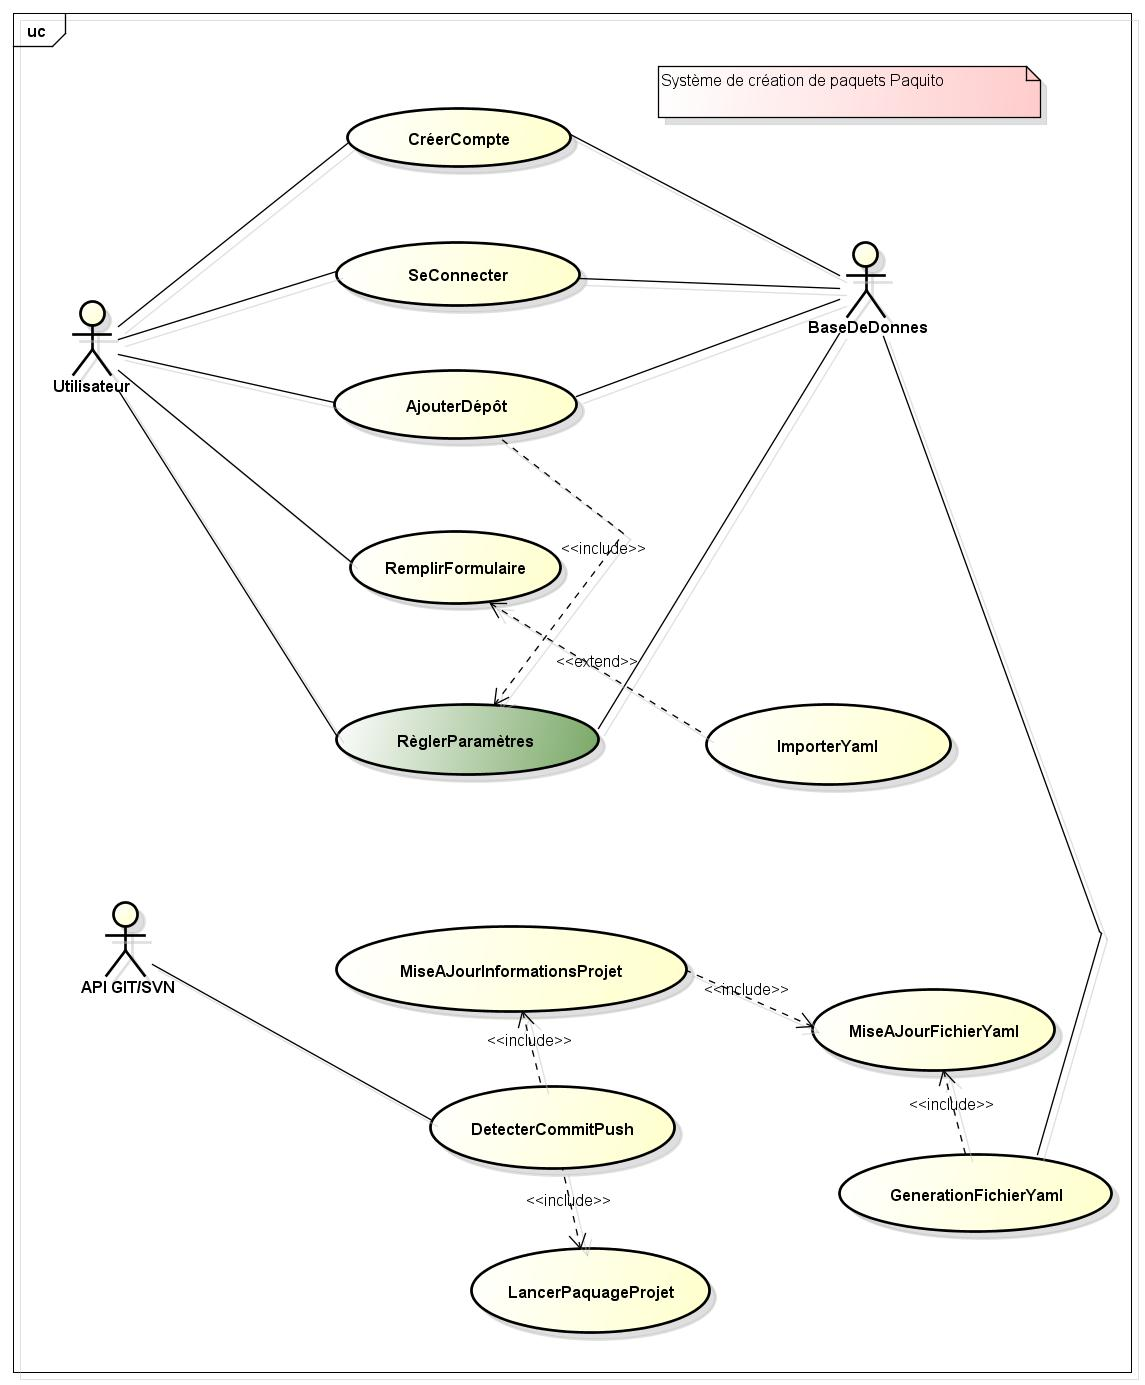
\includegraphics[scale=\largeur]{../img/Diagram_reglerParametre.jpg}
    \end{flushleft}
  \end{minipage}
  \hfill
  \begin{minipage}{0.5\textwidth}
    \begin{flushright}
      On peut modifier les paramètres de création des paquets
    \end{flushright}
  \end{minipage}
\end{frame}

\begin{frame}{Lancement du paquetage du projet}
  \begin{minipage}{0.40\textwidth}
    \begin{flushleft}
      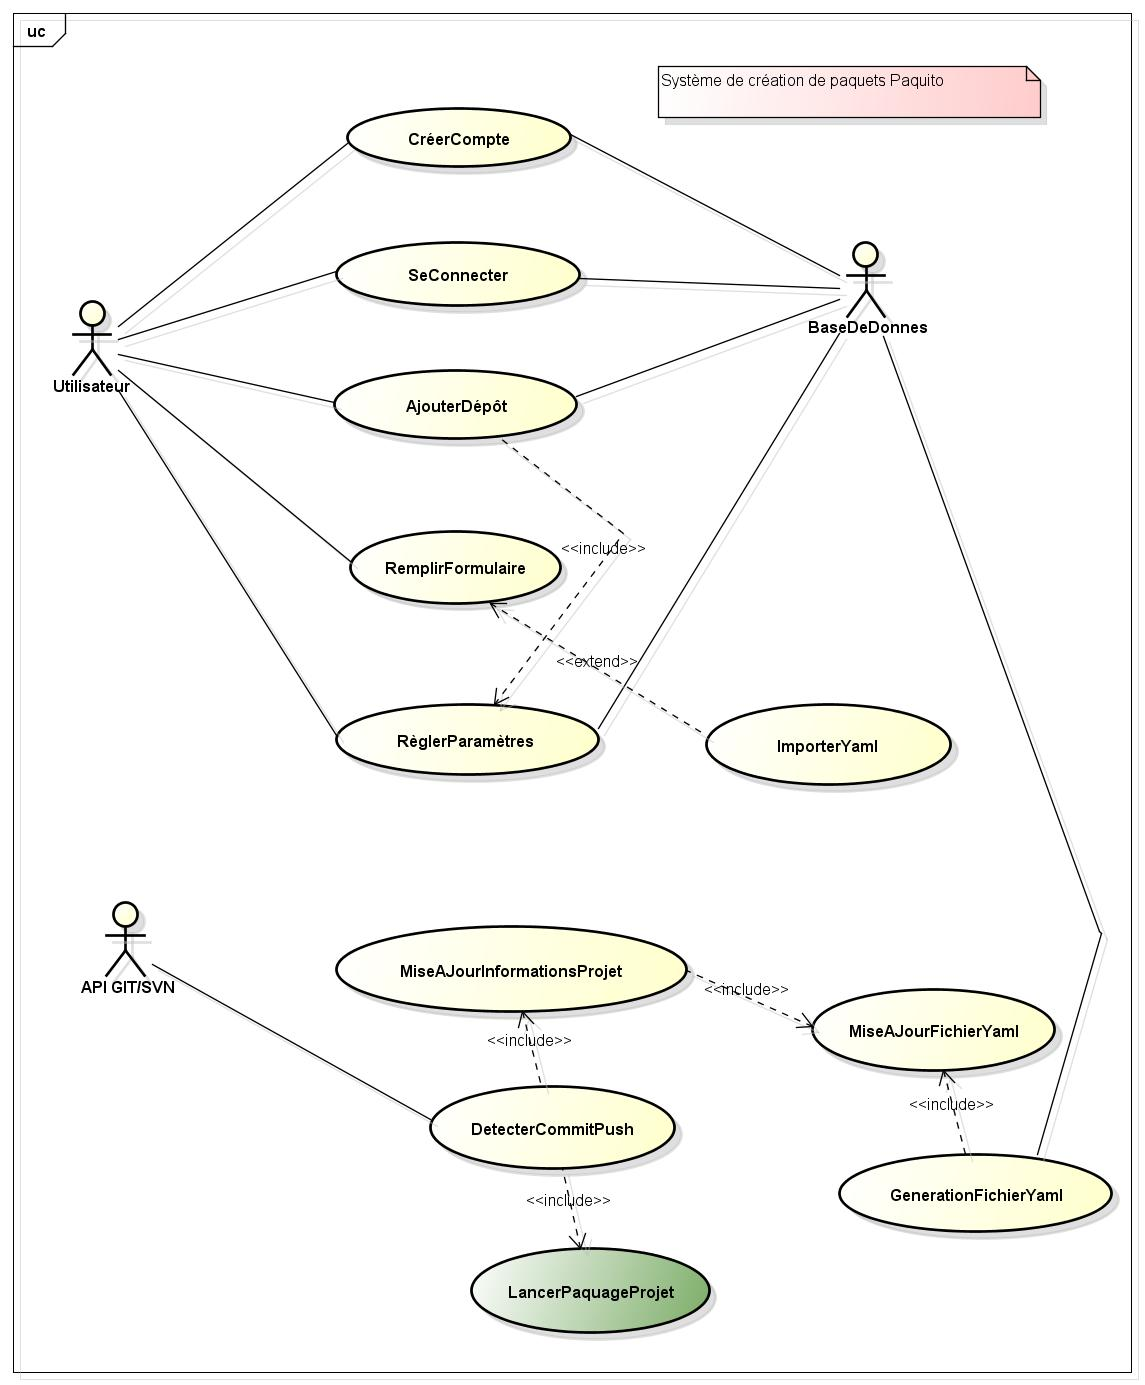
\includegraphics[scale=\largeur]{../img/Diagram_lancerPaquetageProjet.jpg}
    \end{flushleft}
  \end{minipage}
  \hfill
  \begin{minipage}{0.50\textwidth}
    \begin{flushright}
      \begin{itemize}
      \item \textbf{Identification}
        \begin{itemize}
        \item[] Niveau de l'action : Sous fonction
        %\item[] But : Créer les fichiers qui composent le paquetage et genère le fichier contenant les informations sur le paquetage
        \item[] Acteur : API GIT/SVN
        \end{itemize}
      \item \textbf{Scénario principal}
        \begin{enumerate}
        \item Les sources et le fichier YAML ainsi que d'autres informations sont envoyées, via ssh par exemple, aux Machines Virtuelles.
        \item Lancement de l'opération de compilation.
        \item On notifie le(s) développeur(s) de la réussite de la création du paquetage
        \end{enumerate}
      \item \textbf{Echec}
        \begin{itemize}
        \item En cas d'erreur lors de la création du paquetage on envoie une notification au(x) développeur(s) avec l'erreur retournée par Paquito
        \end{itemize}
      \end{itemize}
    \end{flushright}
  \end{minipage}
\end{frame}

\begin{frame}{Détection de Commit ou de Push}
  \begin{minipage}{0.40\textwidth}
    \begin{flushleft}
      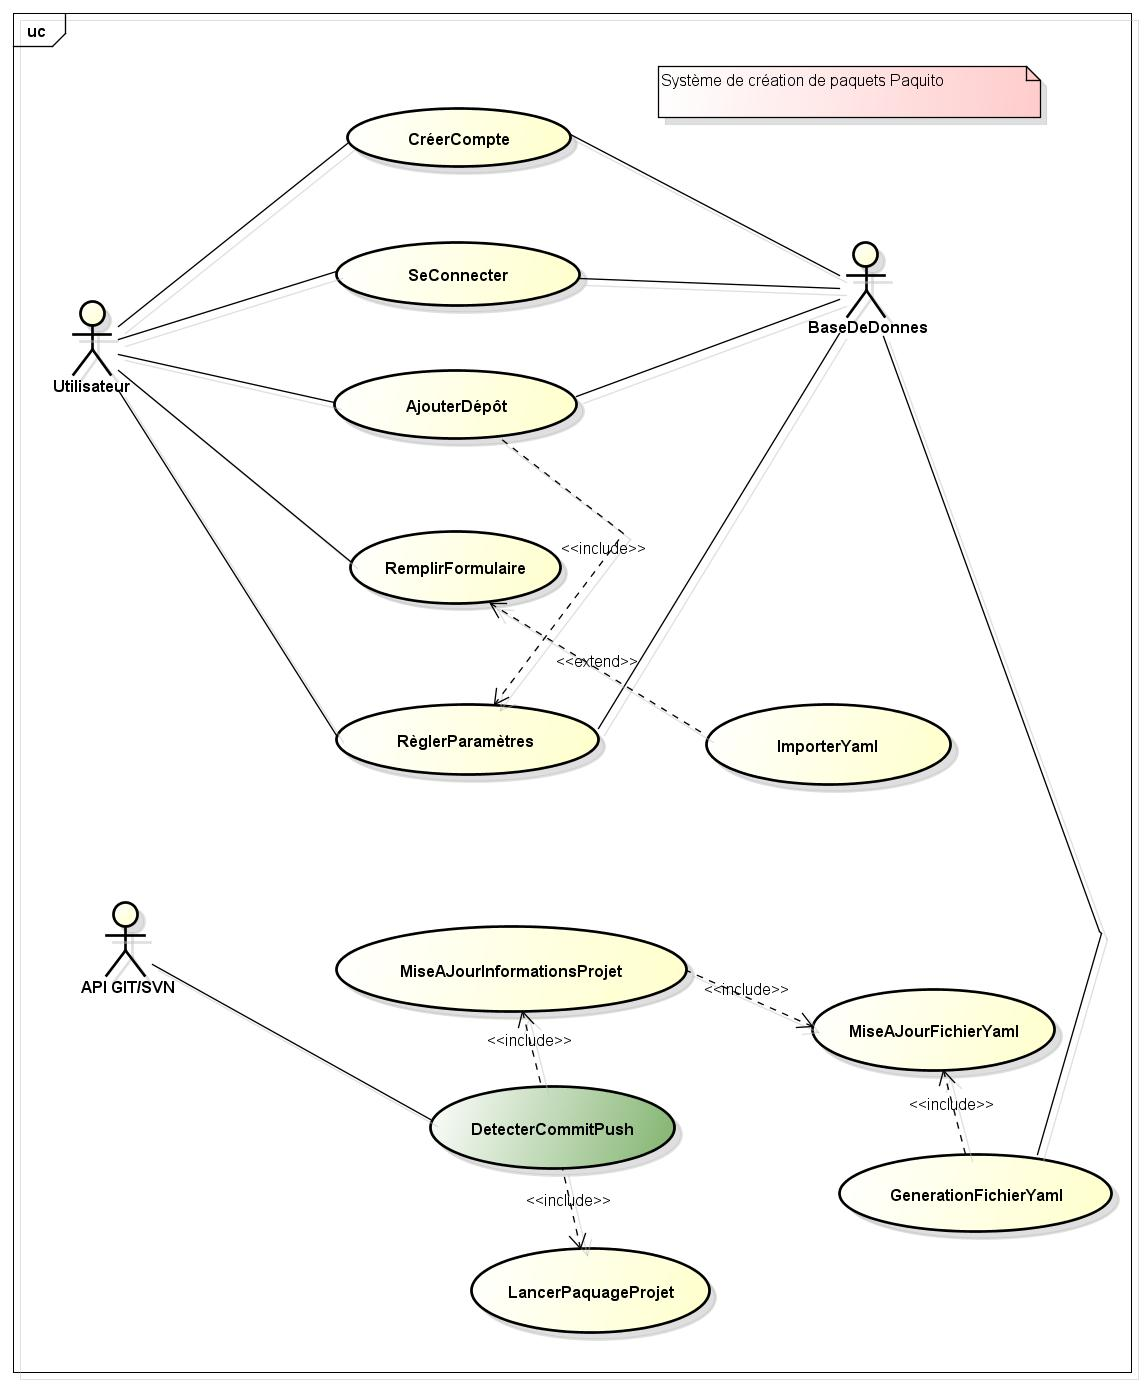
\includegraphics[scale=\largeur]{../img/Diagram_detecterCommitPush.jpg}
    \end{flushleft}
  \end{minipage}
  \hfill
  \begin{minipage}{0.5\textwidth}
    \begin{flushright}
      \begin{itemize}
      \item \textbf{Identification}
        \begin{itemize}
        \item[] Niveau de l'action : Sous fonction
        %\item[] But : L’API GIT/SVN détecte un changement, qui est notamment un commit ou un push.
        \item[] Acteur : API GIT/ SVN
        \end{itemize}
      \item \textbf{Scénario principal}
        \begin{enumerate}
        \item Un développeur fait un commit/push sur son dépôt.
        \item Le serveur en est averti via l’API Git/Svn
        \item Les informations du projet ont été mises à jour
        \item Lancement de la compilation et paquetage sur les Machines Virtuelles du projet.
        \end{enumerate}
      \end{itemize}
    \end{flushright}
  \end{minipage}
\end{frame}

\begin{frame}{Remplir formulaire}
  \begin{minipage}{0.40\textwidth}
    \begin{flushleft}
      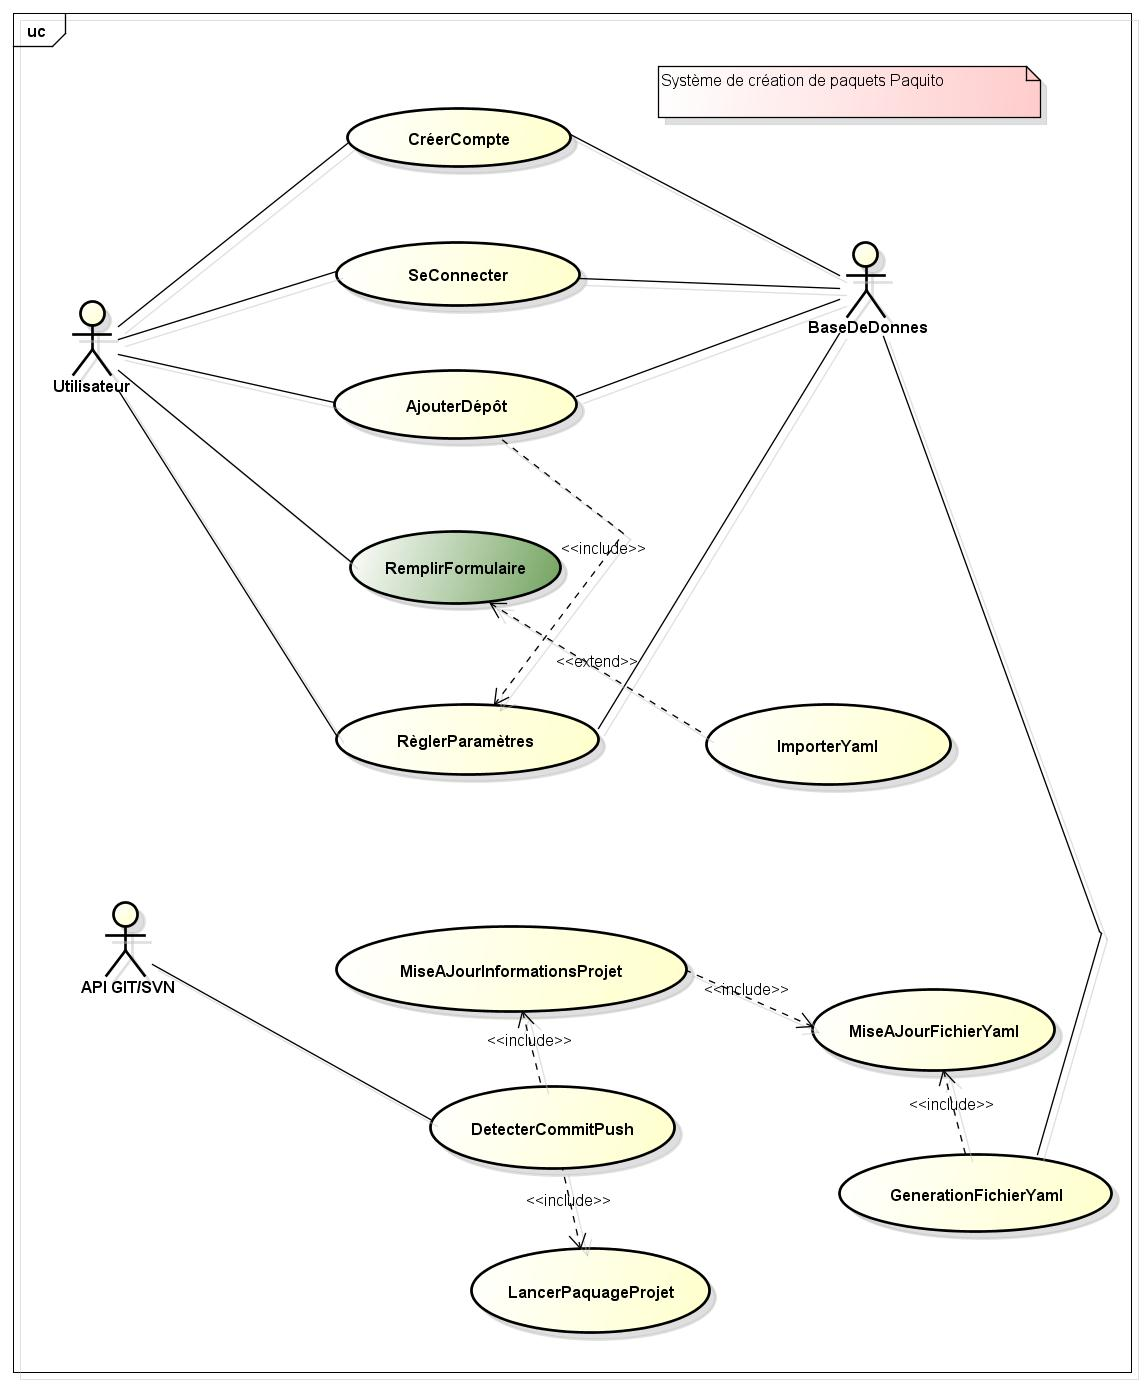
\includegraphics[scale=\largeur]{../img/Diagram_remplirFormulaire.jpg}
    \end{flushleft}
  \end{minipage}
  \hfill
  \begin{minipage}{0.5\textwidth}
    \begin{flushright}
      \begin{itemize}
      \item \textbf{Identification}
        \begin{itemize}
        \item[] Niveau de l'action : Sous fonction
        %\item[] But : L'utilisateur rempli les informations sur le projet qu'il veut faire suivre par paquito
        \item[] Acteur : Utilisateur
        \end{itemize}
      \item \textbf{Scénario principal}
        \begin{enumerate}
        \item L'utilisateur rempli tous les champs
        \item L'utilisateur soumet le formulaire
        \end{enumerate}
      \item \textbf{Echec}
        \begin{itemize}
        \item Un ou plusieurs champs ne sont pas remplis
        \end{itemize}
      \end{itemize}
    \end{flushright}
  \end{minipage}
\end{frame}

\begin{frame}{Importer un fichier YAML}
  \begin{minipage}{0.40\textwidth}
    \begin{flushleft}
      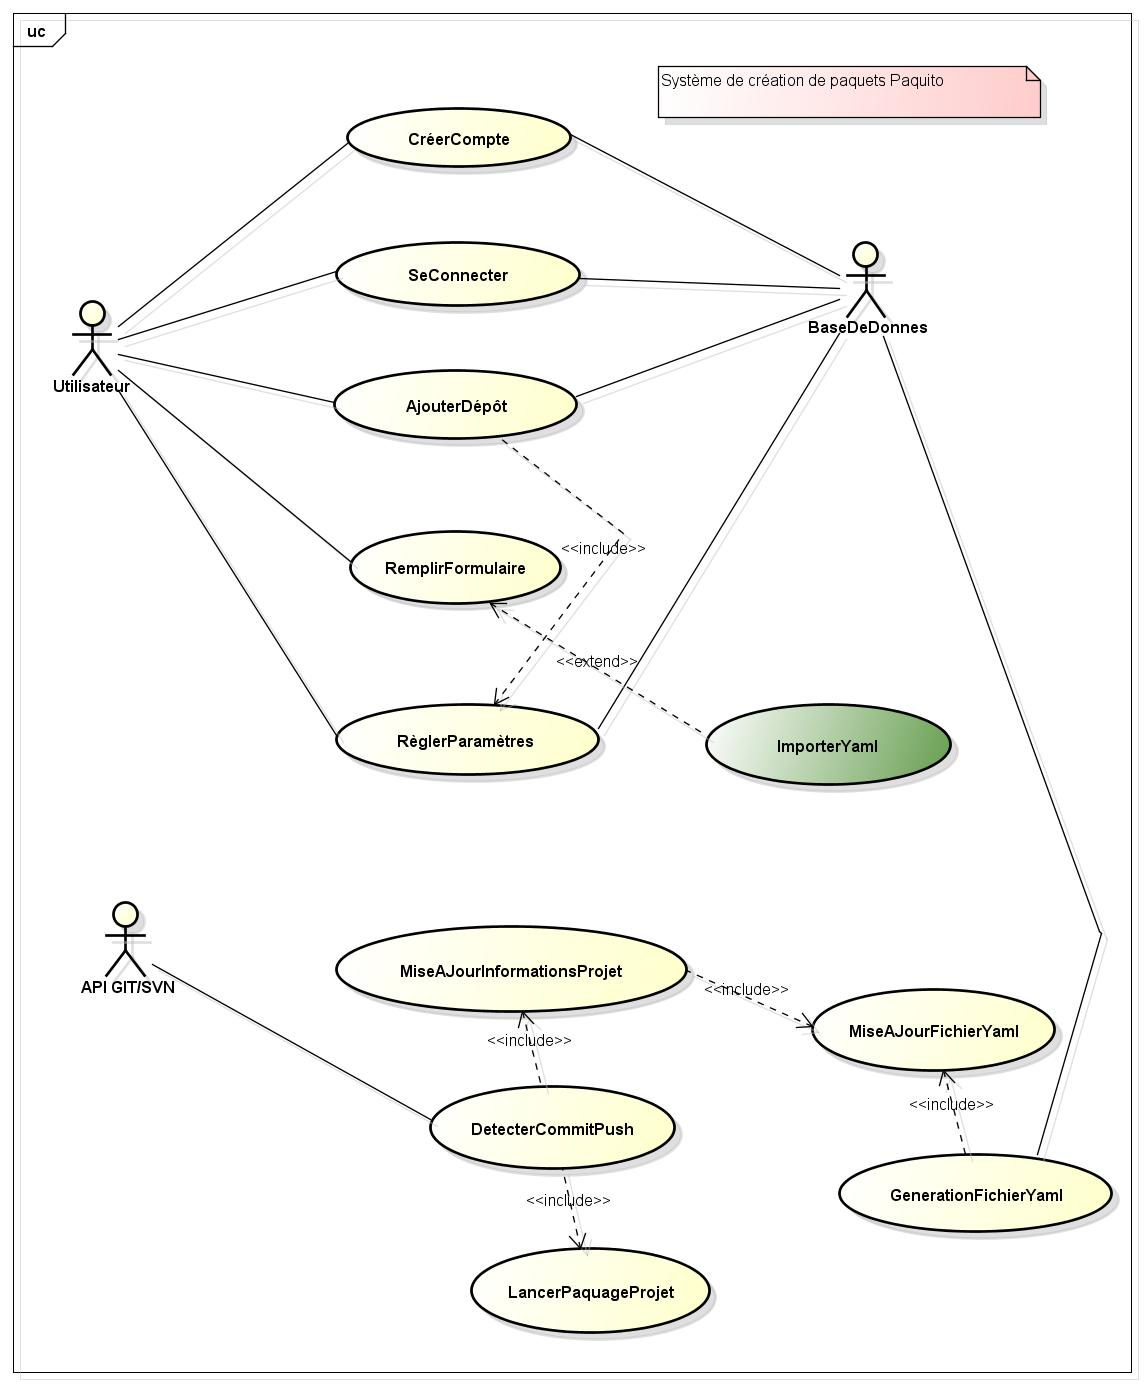
\includegraphics[scale=\largeur]{../img/Diagram_importerYaml.jpg}
    \end{flushleft}
  \end{minipage}
  \hfill
  \begin{minipage}{0.5\textwidth}
    \begin{flushright}
      \begin{itemize}
      \item \textbf{Identification}
        \begin{itemize}
        \item[] Niveau de l'action : Sous-fonction
        %\item[] But : Importer un fichier YAML lorsque le développeur l'a déjà en sa disposition
        \item[] Acteur : Utilisateur
        \end{itemize}
      \item \textbf{Scénario principal}
        \begin{enumerate}
        \item Le développeur va envoyer son fichier YAML via l'application Web
        \item Le système va lire le fichier et remplir automatiquement le formulaire sur l'application Web.
        \end{enumerate}
      \end{itemize}
    \end{flushright}
  \end{minipage}
\end{frame}

\renewcommand\largeur{0.485}

\section{Base de données}
\begin{frame}{Base de données}
  \begin{center}
    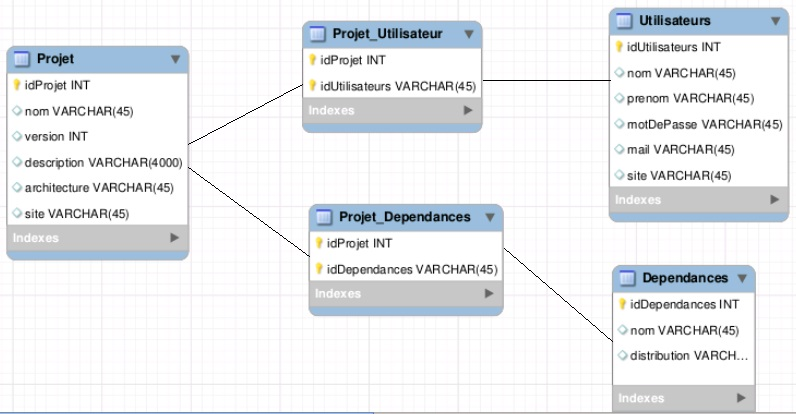
\includegraphics[scale=0.65]{../img/bdd.jpg}
  \end{center}
\end{frame}

\section{Interface web}
\begin{frame}{Page de connexion et d'inscription}
  \begin{center}
    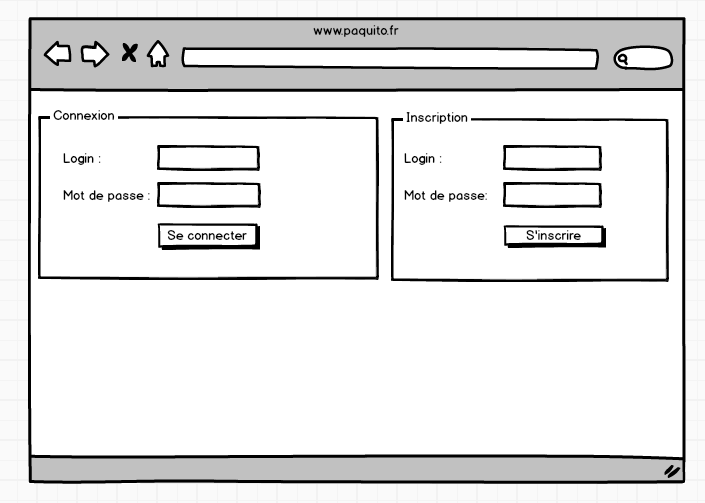
\includegraphics[scale=\largeur]{../img/connexionPaquito.png}
  \end{center}
\end{frame}

\begin{frame}{Page d'ajout d'un projet à Paquito}
  \begin{center}
    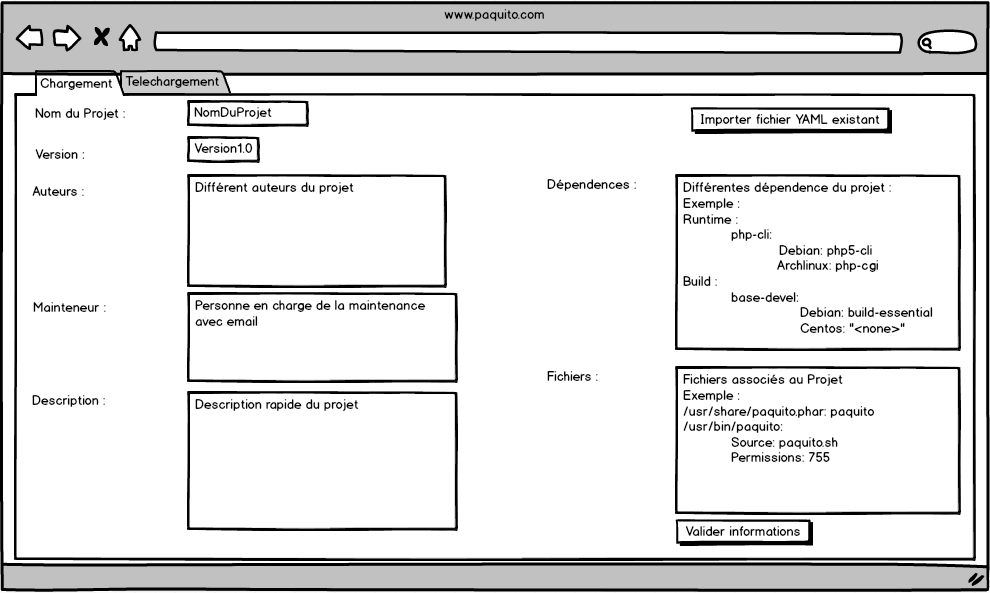
\includegraphics[scale=0.4]{../img/ajouterProjet.png}
  \end{center}
\end{frame}

\begin{frame}{Page de résumé d'un projet}
  \begin{center}
    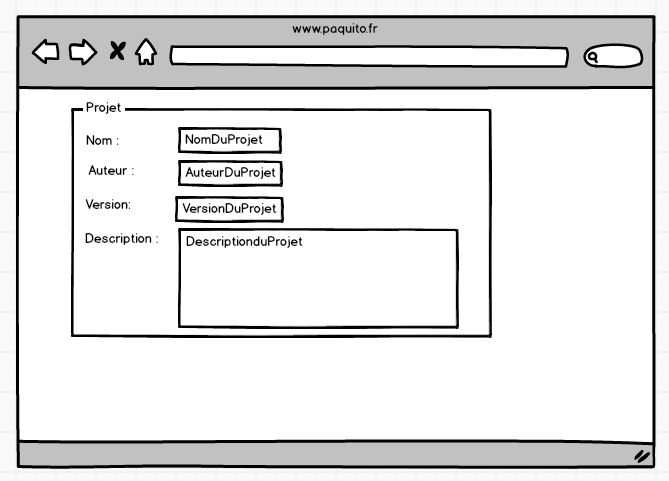
\includegraphics[scale=\largeur]{../img/resumeProjet.png}
  \end{center}
\end{frame}

\begin{frame}{Page de téléchargement d'un projet}
  \begin{center}
    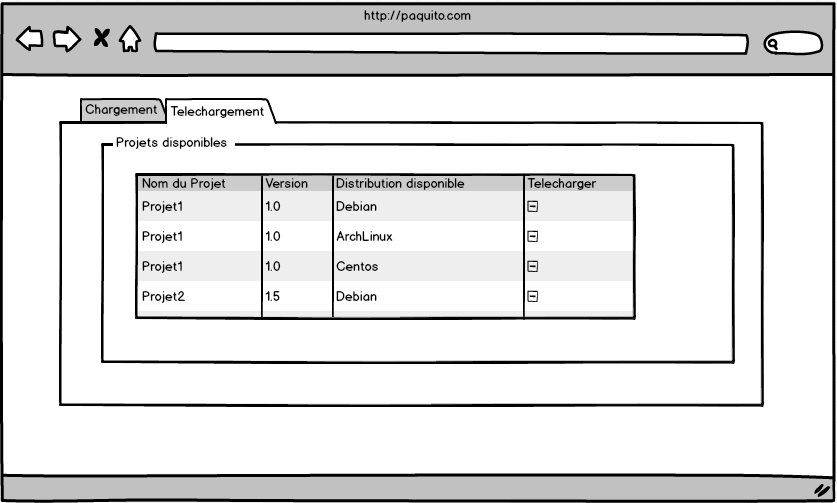
\includegraphics[scale=\largeur]{../img/telechargerProjet.png}
  \end{center}
\end{frame}

\section*{Conclusion}
\begin{frame}{Conclusion}
	\begin{center}
		
\includegraphics[scale=0.1]{../img/paquito.png}
	
		Merci de nous avoir écoutés. 

	\end{center}
\end{frame}

\end{document}
